\documentclass{book}
\usepackage[a4paper,top=2.5cm,bottom=2.5cm,left=2.5cm,right=2.5cm]{geometry}
\usepackage{makeidx}
\usepackage{natbib}
\usepackage{graphicx}
\usepackage{multicol}
\usepackage{float}
\usepackage{listings}
\usepackage{color}
\usepackage{ifthen}
\usepackage[table]{xcolor}
\usepackage{textcomp}
\usepackage{alltt}
\usepackage{ifpdf}
\ifpdf
\usepackage[pdftex,
            pagebackref=true,
            colorlinks=true,
            linkcolor=blue,
            unicode
           ]{hyperref}
\else
\usepackage[ps2pdf,
            pagebackref=true,
            colorlinks=true,
            linkcolor=blue,
            unicode
           ]{hyperref}
\usepackage{pspicture}
\fi
\usepackage[utf8]{inputenc}
\usepackage{mathptmx}
\usepackage[scaled=.90]{helvet}
\usepackage{courier}
\usepackage{sectsty}
\usepackage{amssymb}
\usepackage[titles]{tocloft}
\usepackage{doxygen}
\lstset{language=C++,inputencoding=utf8,basicstyle=\footnotesize,breaklines=true,breakatwhitespace=true,tabsize=4,numbers=left }
\makeindex
\setcounter{tocdepth}{3}
\renewcommand{\footrulewidth}{0.4pt}
\renewcommand{\familydefault}{\sfdefault}
\hfuzz=15pt
\setlength{\emergencystretch}{15pt}
\hbadness=750
\tolerance=750
\begin{document}
\hypersetup{pageanchor=false,citecolor=blue}
\begin{titlepage}
\vspace*{7cm}
\begin{center}
{\Large C\-A\-L\-\_\-\-Grafos \\[1ex]\large 1.\-0 }\\
\vspace*{1cm}
{\large Generated by Doxygen 1.8.3.1}\\
\vspace*{0.5cm}
{\small Fri Apr 26 2013 11:16:26}\\
\end{center}
\end{titlepage}
\clearemptydoublepage
\pagenumbering{roman}
\tableofcontents
\clearemptydoublepage
\pagenumbering{arabic}
\hypersetup{pageanchor=true,citecolor=blue}
\chapter{Hierarchical Index}
\section{Class Hierarchy}
This inheritance list is sorted roughly, but not completely, alphabetically\-:\begin{DoxyCompactList}
\item \contentsline{section}{Client}{\pageref{classClient}}{}
\item \contentsline{section}{Connection}{\pageref{classConnection}}{}
\item \contentsline{section}{Edge$<$ T $>$}{\pageref{classEdge}}{}
\item \contentsline{section}{edge\-\_\-greater\-\_\-than$<$ T $>$}{\pageref{structedge__greater__than}}{}
\item \contentsline{section}{Edge\-Type}{\pageref{classEdgeType}}{}
\item \contentsline{section}{Graph$<$ T $>$}{\pageref{classGraph}}{}
\item \contentsline{section}{Graph$<$ int $>$}{\pageref{classGraph}}{}
\begin{DoxyCompactList}
\item \contentsline{section}{Map}{\pageref{classMap}}{}
\end{DoxyCompactList}
\item \contentsline{section}{Graph\-Viewer}{\pageref{classGraphViewer}}{}
\item \contentsline{section}{Vertex$<$ T $>$}{\pageref{classVertex}}{}
\item \contentsline{section}{Vertex$<$ int $>$}{\pageref{classVertex}}{}
\begin{DoxyCompactList}
\item \contentsline{section}{Zone}{\pageref{classZone}}{}
\end{DoxyCompactList}
\item \contentsline{section}{vertex\-\_\-greater\-\_\-than$<$ T $>$}{\pageref{structvertex__greater__than}}{}
\end{DoxyCompactList}

\chapter{Class Index}
\section{Class List}
Here are the classes, structs, unions and interfaces with brief descriptions\-:\begin{DoxyCompactList}
\item\contentsline{section}{\hyperlink{classClient}{Client} \\*Represests a client in the graph. Stores name, N\-I\-F, zone and store zone }{\pageref{classClient}}{}
\item\contentsline{section}{\hyperlink{classConnection}{Connection} }{\pageref{classConnection}}{}
\item\contentsline{section}{\hyperlink{classEdge}{Edge$<$ T $>$} }{\pageref{classEdge}}{}
\item\contentsline{section}{\hyperlink{structedge__greater__than}{edge\-\_\-greater\-\_\-than$<$ T $>$} }{\pageref{structedge__greater__than}}{}
\item\contentsline{section}{\hyperlink{classEdgeType}{Edge\-Type} }{\pageref{classEdgeType}}{}
\item\contentsline{section}{\hyperlink{classGraph}{Graph$<$ T $>$} }{\pageref{classGraph}}{}
\item\contentsline{section}{\hyperlink{classGraphViewer}{Graph\-Viewer} }{\pageref{classGraphViewer}}{}
\item\contentsline{section}{\hyperlink{classMap}{Map} \\*Represents map. Inherits \hyperlink{classGraph}{Graph} class }{\pageref{classMap}}{}
\item\contentsline{section}{\hyperlink{classVertex}{Vertex$<$ T $>$} }{\pageref{classVertex}}{}
\item\contentsline{section}{\hyperlink{structvertex__greater__than}{vertex\-\_\-greater\-\_\-than$<$ T $>$} }{\pageref{structvertex__greater__than}}{}
\item\contentsline{section}{\hyperlink{classZone}{Zone} \\*Represents a \hyperlink{classZone}{Zone} in which there may or may not be a store }{\pageref{classZone}}{}
\end{DoxyCompactList}

\chapter{Class Documentation}
\hypertarget{classClient}{\section{Client Class Reference}
\label{classClient}\index{Client@{Client}}
}


Represests a client in the graph. Stores name, N\-I\-F, zone and store zone.  




{\ttfamily \#include $<$Client.\-h$>$}

\subsection*{Public Member Functions}
\begin{DoxyCompactItemize}
\item 
\hyperlink{classClient_a536244b1fef9e107769dd1e626606994}{Client} (string name, unsigned long N\-I\-F)
\begin{DoxyCompactList}\small\item\em \hyperlink{classClient}{Client} constructor. Initially it does not have a set sone or store zone so it can be determined later. \end{DoxyCompactList}\item 
string \hyperlink{classClient_aa2eff010fd1f9ac7bab938b8d432b55f}{get\-Name} ()
\begin{DoxyCompactList}\small\item\em Gets client name. \end{DoxyCompactList}\item 
unsigned long \hyperlink{classClient_a059dedac3349c4b07a03de76a613ed26}{get\-N\-I\-F} ()
\begin{DoxyCompactList}\small\item\em Gets client N\-I\-F. \end{DoxyCompactList}\item 
int \hyperlink{classClient_aa0d1054fb50575f0b2a8469d6fa4acf9}{get\-Zone} ()
\begin{DoxyCompactList}\small\item\em Gets client zone. \end{DoxyCompactList}\item 
void \hyperlink{classClient_ad92d3d3c599e9662378c41b7937cf568}{set\-Zone} (int zone)
\begin{DoxyCompactList}\small\item\em Sets client zone. \end{DoxyCompactList}\item 
void \hyperlink{classClient_a440b60950611f1ac80116fb2e6edfea6}{set\-Store\-Zone} (int zone)
\begin{DoxyCompactList}\small\item\em Sets \hyperlink{classClient}{Client}'s store zone. \end{DoxyCompactList}\end{DoxyCompactItemize}
\subsection*{Public Attributes}
\begin{DoxyCompactItemize}
\item 
\hypertarget{classClient_a35ca221fe5a0449205832555163774ac}{int {\bfseries store\-Zone}}\label{classClient_a35ca221fe5a0449205832555163774ac}

\end{DoxyCompactItemize}


\subsection{Detailed Description}
Represests a client in the graph. Stores name, N\-I\-F, zone and store zone. 

\subsection{Constructor \& Destructor Documentation}
\hypertarget{classClient_a536244b1fef9e107769dd1e626606994}{\index{Client@{Client}!Client@{Client}}
\index{Client@{Client}!Client@{Client}}
\subsubsection[{Client}]{\setlength{\rightskip}{0pt plus 5cm}Client\-::\-Client (
\begin{DoxyParamCaption}
\item[{string}]{name, }
\item[{unsigned long}]{N\-I\-F}
\end{DoxyParamCaption}
)}}\label{classClient_a536244b1fef9e107769dd1e626606994}


\hyperlink{classClient}{Client} constructor. Initially it does not have a set sone or store zone so it can be determined later. 


\begin{DoxyParams}{Parameters}
{\em name} & \hyperlink{classClient}{Client}'s name \\
\hline
{\em N\-I\-F} & \hyperlink{classClient}{Client}'s N\-I\-F \\
\hline
\end{DoxyParams}


\subsection{Member Function Documentation}
\hypertarget{classClient_aa2eff010fd1f9ac7bab938b8d432b55f}{\index{Client@{Client}!get\-Name@{get\-Name}}
\index{get\-Name@{get\-Name}!Client@{Client}}
\subsubsection[{get\-Name}]{\setlength{\rightskip}{0pt plus 5cm}string Client\-::get\-Name (
\begin{DoxyParamCaption}
{}
\end{DoxyParamCaption}
)}}\label{classClient_aa2eff010fd1f9ac7bab938b8d432b55f}


Gets client name. 

\begin{DoxyReturn}{Returns}
\hyperlink{classClient}{Client} name 
\end{DoxyReturn}
\hypertarget{classClient_a059dedac3349c4b07a03de76a613ed26}{\index{Client@{Client}!get\-N\-I\-F@{get\-N\-I\-F}}
\index{get\-N\-I\-F@{get\-N\-I\-F}!Client@{Client}}
\subsubsection[{get\-N\-I\-F}]{\setlength{\rightskip}{0pt plus 5cm}unsigned long Client\-::get\-N\-I\-F (
\begin{DoxyParamCaption}
{}
\end{DoxyParamCaption}
)}}\label{classClient_a059dedac3349c4b07a03de76a613ed26}


Gets client N\-I\-F. 

\begin{DoxyReturn}{Returns}
\hyperlink{classClient}{Client} N\-I\-F 
\end{DoxyReturn}
\hypertarget{classClient_aa0d1054fb50575f0b2a8469d6fa4acf9}{\index{Client@{Client}!get\-Zone@{get\-Zone}}
\index{get\-Zone@{get\-Zone}!Client@{Client}}
\subsubsection[{get\-Zone}]{\setlength{\rightskip}{0pt plus 5cm}int Client\-::get\-Zone (
\begin{DoxyParamCaption}
{}
\end{DoxyParamCaption}
)}}\label{classClient_aa0d1054fb50575f0b2a8469d6fa4acf9}


Gets client zone. 

\begin{DoxyReturn}{Returns}
\hyperlink{classClient}{Client} zone 
\end{DoxyReturn}
\hypertarget{classClient_a440b60950611f1ac80116fb2e6edfea6}{\index{Client@{Client}!set\-Store\-Zone@{set\-Store\-Zone}}
\index{set\-Store\-Zone@{set\-Store\-Zone}!Client@{Client}}
\subsubsection[{set\-Store\-Zone}]{\setlength{\rightskip}{0pt plus 5cm}void Client\-::set\-Store\-Zone (
\begin{DoxyParamCaption}
\item[{int}]{zone}
\end{DoxyParamCaption}
)}}\label{classClient_a440b60950611f1ac80116fb2e6edfea6}


Sets \hyperlink{classClient}{Client}'s store zone. 


\begin{DoxyParams}{Parameters}
{\em zone} & \hyperlink{classClient}{Client}'s store zone \\
\hline
\end{DoxyParams}
\hypertarget{classClient_ad92d3d3c599e9662378c41b7937cf568}{\index{Client@{Client}!set\-Zone@{set\-Zone}}
\index{set\-Zone@{set\-Zone}!Client@{Client}}
\subsubsection[{set\-Zone}]{\setlength{\rightskip}{0pt plus 5cm}void Client\-::set\-Zone (
\begin{DoxyParamCaption}
\item[{int}]{zone}
\end{DoxyParamCaption}
)}}\label{classClient_ad92d3d3c599e9662378c41b7937cf568}


Sets client zone. 


\begin{DoxyParams}{Parameters}
{\em zone} & \hyperlink{classClient}{Client} zone \\
\hline
\end{DoxyParams}


The documentation for this class was generated from the following files\-:\begin{DoxyCompactItemize}
\item 
Client.\-h\item 
Client.\-cpp\end{DoxyCompactItemize}

\hypertarget{classConnection}{\section{Connection Class Reference}
\label{classConnection}\index{Connection@{Connection}}
}
\subsection*{Public Member Functions}
\begin{DoxyCompactItemize}
\item 
\hypertarget{classConnection_a8089476d48ba545f44e691cd4bd0278d}{{\bfseries Connection} (short port)}\label{classConnection_a8089476d48ba545f44e691cd4bd0278d}

\item 
\hypertarget{classConnection_a4b9f6db1fb42fc9857f829fa0bc52e6e}{bool {\bfseries send\-Msg} (string msg)}\label{classConnection_a4b9f6db1fb42fc9857f829fa0bc52e6e}

\item 
\hypertarget{classConnection_a1df16b436751b686d96c24ca0c498659}{string {\bfseries read\-Line} ()}\label{classConnection_a1df16b436751b686d96c24ca0c498659}

\end{DoxyCompactItemize}


The documentation for this class was generated from the following files\-:\begin{DoxyCompactItemize}
\item 
Connection.\-h\item 
Connection.\-cpp\end{DoxyCompactItemize}

\hypertarget{classEdge}{\section{Edge$<$ T $>$ Class Template Reference}
\label{classEdge}\index{Edge$<$ T $>$@{Edge$<$ T $>$}}
}
\subsection*{Public Member Functions}
\begin{DoxyCompactItemize}
\item 
\hypertarget{classEdge_a9e1bb0df9fbcf5471a745d55b21d7d60}{{\bfseries Edge} (\hyperlink{classVertex}{Vertex}$<$ T $>$ $\ast$d, double w, double f=0)}\label{classEdge_a9e1bb0df9fbcf5471a745d55b21d7d60}

\item 
\hypertarget{classEdge_ac825bb839c49eac8b9c0c56cbd8ff31d}{double {\bfseries get\-Flow} () const }\label{classEdge_ac825bb839c49eac8b9c0c56cbd8ff31d}

\item 
\hypertarget{classEdge_a78f814ec429f84cd7336402326ad4ea8}{double {\bfseries get\-Weight} () const }\label{classEdge_a78f814ec429f84cd7336402326ad4ea8}

\item 
\hypertarget{classEdge_a3805fa2e04f1e7f0495fbba6524ea823}{\hyperlink{classVertex}{Vertex}$<$ T $>$ $\ast$ {\bfseries get\-Dest} () const }\label{classEdge_a3805fa2e04f1e7f0495fbba6524ea823}

\item 
\hypertarget{classEdge_a508b08c169f786a48652dc818fb442cd}{bool {\bfseries operator$<$} (const \hyperlink{classEdge}{Edge}$<$ T $>$ \&other) const }\label{classEdge_a508b08c169f786a48652dc818fb442cd}

\end{DoxyCompactItemize}
\subsection*{Public Attributes}
\begin{DoxyCompactItemize}
\item 
\hypertarget{classEdge_ae4d65678b91bd9d814af4720ad87cd0c}{\hyperlink{classVertex}{Vertex}$<$ T $>$ $\ast$ {\bfseries dest}}\label{classEdge_ae4d65678b91bd9d814af4720ad87cd0c}

\item 
\hypertarget{classEdge_a4510c31e0479f9d25f6e35d086887192}{\hyperlink{classVertex}{Vertex}$<$ T $>$ $\ast$ {\bfseries orig}}\label{classEdge_a4510c31e0479f9d25f6e35d086887192}

\item 
\hypertarget{classEdge_af188b57b604f0d65e2da48733bd76426}{double {\bfseries weight}}\label{classEdge_af188b57b604f0d65e2da48733bd76426}

\item 
\hypertarget{classEdge_a30808601fa37f509147eabf9cc5f9ed6}{double {\bfseries flow}}\label{classEdge_a30808601fa37f509147eabf9cc5f9ed6}

\end{DoxyCompactItemize}
\subsection*{Friends}
\begin{DoxyCompactItemize}
\item 
\hypertarget{classEdge_aefa9b76cd57411c5354e5620dc2d84dd}{class {\bfseries Graph$<$ T $>$}}\label{classEdge_aefa9b76cd57411c5354e5620dc2d84dd}

\item 
\hypertarget{classEdge_a2e120a12dec663fa334633b4f26cbed8}{class {\bfseries Vertex$<$ T $>$}}\label{classEdge_a2e120a12dec663fa334633b4f26cbed8}

\end{DoxyCompactItemize}


The documentation for this class was generated from the following file\-:\begin{DoxyCompactItemize}
\item 
Graph.\-h\end{DoxyCompactItemize}

\hypertarget{structedge__greater__than}{\section{edge\-\_\-greater\-\_\-than$<$ T $>$ Struct Template Reference}
\label{structedge__greater__than}\index{edge\-\_\-greater\-\_\-than$<$ T $>$@{edge\-\_\-greater\-\_\-than$<$ T $>$}}
}
\subsection*{Public Member Functions}
\begin{DoxyCompactItemize}
\item 
\hypertarget{structedge__greater__than_a364f16a857cc5061530aac6c7b02bba4}{bool {\bfseries operator()} (\hyperlink{classEdge}{Edge}$<$ T $>$ a, \hyperlink{classEdge}{Edge}$<$ T $>$ b) const }\label{structedge__greater__than_a364f16a857cc5061530aac6c7b02bba4}

\end{DoxyCompactItemize}


The documentation for this struct was generated from the following file\-:\begin{DoxyCompactItemize}
\item 
Graph.\-h\end{DoxyCompactItemize}

\hypertarget{classEdgeType}{\section{Edge\-Type Class Reference}
\label{classEdgeType}\index{Edge\-Type@{Edge\-Type}}
}


{\ttfamily \#include $<$Edgetype.\-h$>$}

\subsection*{Static Public Attributes}
\begin{DoxyCompactItemize}
\item 
\hypertarget{classEdgeType_a6533cc56d05c288a550b9980b66c9317}{static const int {\bfseries U\-N\-D\-I\-R\-E\-C\-T\-E\-D} = 0}\label{classEdgeType_a6533cc56d05c288a550b9980b66c9317}

\item 
\hypertarget{classEdgeType_a903017a534f2818c2d17145e4ae0321c}{static const int {\bfseries D\-I\-R\-E\-C\-T\-E\-D} = 1}\label{classEdgeType_a903017a534f2818c2d17145e4ae0321c}

\end{DoxyCompactItemize}


\subsection{Detailed Description}
Classe que enumera os tipos de arestas. Usar Edge\-Type.\-U\-N\-D\-I\-R\-E\-C\-T\-E\-D para uma aresta sem direcção, ou Edge\-Type.\-D\-I\-R\-E\-C\-T\-E\-D para uma aresta dirigida. 

The documentation for this class was generated from the following file\-:\begin{DoxyCompactItemize}
\item 
Edgetype.\-h\end{DoxyCompactItemize}

\hypertarget{classGraph}{\section{Graph$<$ T $>$ Class Template Reference}
\label{classGraph}\index{Graph$<$ T $>$@{Graph$<$ T $>$}}
}
\subsection*{Public Member Functions}
\begin{DoxyCompactItemize}
\item 
\hypertarget{classGraph_a00be284ea2be3b3d0f0d2e493b70245b}{bool {\bfseries add\-Vertex} (const T \&in)}\label{classGraph_a00be284ea2be3b3d0f0d2e493b70245b}

\item 
\hypertarget{classGraph_a78d952c4aa7ca2b828c1042b12995069}{bool {\bfseries add\-Edge} (const T \&sourc, const T \&dest, double w, double f=0)}\label{classGraph_a78d952c4aa7ca2b828c1042b12995069}

\item 
\hypertarget{classGraph_af9c903104ad69a7782979fa9caedf163}{bool {\bfseries remove\-Vertex} (const T \&in)}\label{classGraph_af9c903104ad69a7782979fa9caedf163}

\item 
\hypertarget{classGraph_a1106092a37366486cf55576f9ec01692}{bool {\bfseries remove\-Edge} (const T \&sourc, const T \&dest)}\label{classGraph_a1106092a37366486cf55576f9ec01692}

\item 
\hypertarget{classGraph_a6f66082eeeaef42d51cb7f2e2c3cb6e2}{vector$<$ T $>$ {\bfseries dfs} () const }\label{classGraph_a6f66082eeeaef42d51cb7f2e2c3cb6e2}

\item 
\hypertarget{classGraph_acd33e9b4f345aa28cf73f537ba176e6c}{vector$<$ T $>$ {\bfseries bfs} (\hyperlink{classVertex}{Vertex}$<$ T $>$ $\ast$v) const }\label{classGraph_acd33e9b4f345aa28cf73f537ba176e6c}

\item 
\hypertarget{classGraph_ab8fd74c3cf8dca6eaa82d39fd1216f52}{int {\bfseries max\-New\-Children} (\hyperlink{classVertex}{Vertex}$<$ T $>$ $\ast$v, T \&inf) const }\label{classGraph_ab8fd74c3cf8dca6eaa82d39fd1216f52}

\item 
\hypertarget{classGraph_ab7dc5ec1c34df811d560021b726e95ec}{vector$<$ \hyperlink{classVertex}{Vertex}$<$ T $>$ $\ast$ $>$ {\bfseries get\-Vertex\-Set} () const }\label{classGraph_ab7dc5ec1c34df811d560021b726e95ec}

\item 
\hypertarget{classGraph_a295932f117d92c825a97ec458e0fb332}{int {\bfseries get\-Num\-Vertex} () const }\label{classGraph_a295932f117d92c825a97ec458e0fb332}

\item 
\hypertarget{classGraph_a08a95472b0d9bd7321660940807af060}{\hyperlink{classVertex}{Vertex}$<$ T $>$ $\ast$ {\bfseries get\-Vertex} (const T \&v) const }\label{classGraph_a08a95472b0d9bd7321660940807af060}

\item 
\hypertarget{classGraph_af34eb86d804272e6e3e221a9ed688c53}{void {\bfseries reset\-Indegrees} ()}\label{classGraph_af34eb86d804272e6e3e221a9ed688c53}

\item 
\hypertarget{classGraph_af9502cbf025cc7c7c84d266567d59141}{vector$<$ \hyperlink{classVertex}{Vertex}$<$ T $>$ $\ast$ $>$ {\bfseries get\-Sources} () const }\label{classGraph_af9502cbf025cc7c7c84d266567d59141}

\item 
\hypertarget{classGraph_a694dff81073c38b669057f0c6bd4cbb1}{int {\bfseries get\-Num\-Cycles} ()}\label{classGraph_a694dff81073c38b669057f0c6bd4cbb1}

\item 
\hypertarget{classGraph_ae2305ca51e55cf59fe41735a73e9be09}{vector$<$ T $>$ {\bfseries topological\-Order} ()}\label{classGraph_ae2305ca51e55cf59fe41735a73e9be09}

\item 
\hypertarget{classGraph_ab4054ca572c10669dd3e05d6d41c116c}{vector$<$ T $>$ {\bfseries get\-Path} (const T \&origin, const T \&dest)}\label{classGraph_ab4054ca572c10669dd3e05d6d41c116c}

\item 
\hypertarget{classGraph_ae5264597aacaf4f45819e96a6d6c89aa}{void {\bfseries unweighted\-Shortest\-Path} (const T \&v)}\label{classGraph_ae5264597aacaf4f45819e96a6d6c89aa}

\item 
\hypertarget{classGraph_ab49d07c2bd6b8b30d5ae82bc558b821a}{bool {\bfseries is\-D\-A\-G} ()}\label{classGraph_ab49d07c2bd6b8b30d5ae82bc558b821a}

\item 
\hypertarget{classGraph_a1d6769b79beaa76f78fd9c9209833bef}{void {\bfseries bellman\-Ford\-Shortest\-Path} (const T \&s)}\label{classGraph_a1d6769b79beaa76f78fd9c9209833bef}

\item 
\hypertarget{classGraph_a445a38cf4045797198eae2b818b602de}{void {\bfseries dijkstra\-Shortest\-Path} (const T \&s)}\label{classGraph_a445a38cf4045797198eae2b818b602de}

\item 
\hypertarget{classGraph_ae5161f4408bf1ead2b29d19d67fb04ee}{void {\bfseries floyd\-Warshall\-Shortest\-Path} ()}\label{classGraph_ae5161f4408bf1ead2b29d19d67fb04ee}

\item 
\hypertarget{classGraph_a7e137f1ef838395ac1044a944fa54448}{int {\bfseries edge\-Cost} (int v\-Orig\-Index, int v\-Dest\-Index)}\label{classGraph_a7e137f1ef838395ac1044a944fa54448}

\item 
\hypertarget{classGraph_a8d64c7cae3712215a4d9d7b2a1018444}{vector$<$ T $>$ {\bfseries getfloyd\-Warshall\-Path} (const T \&origin, const T \&dest)}\label{classGraph_a8d64c7cae3712215a4d9d7b2a1018444}

\item 
\hypertarget{classGraph_aad1eda4beb8425d03ed1f3b8af397563}{void {\bfseries getfloyd\-Warshall\-Path\-Aux} (int index1, int index2, vector$<$ T $>$ \&res)}\label{classGraph_aad1eda4beb8425d03ed1f3b8af397563}

\item 
\hypertarget{classGraph_a63c6f899a8bd788cc39c977defd15885}{\hyperlink{classGraph}{Graph}$<$ T $>$ {\bfseries clone} ()}\label{classGraph_a63c6f899a8bd788cc39c977defd15885}

\item 
\hypertarget{classGraph_a8bf372ab4fb01cab6c88f3a2def1d545}{void {\bfseries reset\-Edge\-Flow} ()}\label{classGraph_a8bf372ab4fb01cab6c88f3a2def1d545}

\item 
\hypertarget{classGraph_a0b41e13d9b298f0d89bc7d5c8e902054}{vector$<$ \hyperlink{classVertex}{Vertex}$<$ T $>$ $\ast$ $>$ {\bfseries calculate\-Prim} ()}\label{classGraph_a0b41e13d9b298f0d89bc7d5c8e902054}

\item 
\hypertarget{classGraph_a04426d0a2328f68415192f35a31be9c3}{vector$<$ \hyperlink{classVertex}{Vertex}$<$ T $>$ $\ast$ $>$ {\bfseries calculate\-Kruskal} ()}\label{classGraph_a04426d0a2328f68415192f35a31be9c3}

\end{DoxyCompactItemize}
\subsection*{Public Attributes}
\begin{DoxyCompactItemize}
\item 
\hypertarget{classGraph_a73d4e735fc0a7c83c9c689a2b53fa623}{vector$<$ \hyperlink{classVertex}{Vertex}$<$ T $>$ $\ast$ $>$ {\bfseries vertex\-Set}}\label{classGraph_a73d4e735fc0a7c83c9c689a2b53fa623}

\end{DoxyCompactItemize}


The documentation for this class was generated from the following file\-:\begin{DoxyCompactItemize}
\item 
Graph.\-h\end{DoxyCompactItemize}

\hypertarget{classGraphViewer}{\section{Graph\-Viewer Class Reference}
\label{classGraphViewer}\index{Graph\-Viewer@{Graph\-Viewer}}
}


{\ttfamily \#include $<$Graphviewer.\-h$>$}

\subsection*{Public Member Functions}
\begin{DoxyCompactItemize}
\item 
\hyperlink{classGraphViewer_aefca44052e0000ef416ddafc828f36cc}{Graph\-Viewer} (int width, int height, bool port\-\_\-n)
\item 
\hyperlink{classGraphViewer_ad9d7b1d8b4ba8ef18517eae0e68568a2}{Graph\-Viewer} (int width, int height, bool dynamic, int port\-\_\-n)
\item 
bool \hyperlink{classGraphViewer_ae5247dc66449dcd21fc5d531bbbaddfa}{create\-Window} (int width, int height)
\item 
bool \hyperlink{classGraphViewer_a85990c1eaac7feed3950960d4bd2fd4c}{close\-Window} ()
\item 
bool \hyperlink{classGraphViewer_a5421e86ac76433876309236ba96e70a2}{add\-Node} (int id, int x, int y)
\item 
bool \hyperlink{classGraphViewer_ab9be856eb5f45284719a3bb119ec01ea}{add\-Node} (int id)
\item 
bool \hyperlink{classGraphViewer_aad0c1448c37f744209ffb671f1bd0015}{add\-Edge} (int id, int v1, int v2, int edge\-Type)
\item 
bool \hyperlink{classGraphViewer_a0c418639bb911eb827cabf895915f775}{remove\-Node} (int id)
\item 
bool \hyperlink{classGraphViewer_a9a8ee68c7c12b373affbe4069dd95d72}{remove\-Edge} (int id)
\item 
bool \hyperlink{classGraphViewer_ac25d7d007022fda16799808ba136e909}{set\-Vertex\-Label} (int id, string label)
\item 
bool \hyperlink{classGraphViewer_a447cca0064e785654c2105602c2961ca}{set\-Edge\-Label} (int id, string label)
\item 
bool \hyperlink{classGraphViewer_a07ccc96707efae4aa5f3ced3dca015af}{set\-Edge\-Color} (int id, string color)
\item 
bool \hyperlink{classGraphViewer_a8b542d7e09e81a45a74760c19233beb0}{set\-Vertex\-Color} (int id, string color)
\item 
bool \hyperlink{classGraphViewer_a4102580b69826ba83251ef7bb262f8be}{define\-Edge\-Color} (string color)
\item 
bool \hyperlink{classGraphViewer_a76de8676b7a93d72af514b84cdaa4d21}{define\-Vertex\-Color} (string color)
\item 
bool \hyperlink{classGraphViewer_a07f598272fe3515455eab13be749604a}{set\-Edge\-Thickness} (int id, int thickness)
\item 
bool \hyperlink{classGraphViewer_a02437b5fecd8b90de24436068312d593}{set\-Background} (string path)
\item 
bool \hyperlink{classGraphViewer_ac211de009a0afe2e6d44f4f8d030a2cc}{set\-Edge\-Weight} (int id, int weight)
\item 
bool \hyperlink{classGraphViewer_a69eb065145063e4dea41961e92e35c8e}{set\-Edge\-Flow} (int id, int flow)
\item 
bool \hyperlink{classGraphViewer_a3009a66958686ccb7e78b68e37c3c423}{rearrange} ()
\end{DoxyCompactItemize}
\subsection*{Static Public Attributes}
\begin{DoxyCompactItemize}
\item 
static short \hyperlink{classGraphViewer_a89d0abe75f41feededc49497cc514342}{port} = 7772
\end{DoxyCompactItemize}


\subsection{Detailed Description}
Classe que guarda o grafo e o representa. Todas as suas funções retornam um booleano a indicar se a sua execução decorreu ou não com sucesso. 

\subsection{Constructor \& Destructor Documentation}
\hypertarget{classGraphViewer_aefca44052e0000ef416ddafc828f36cc}{\index{Graph\-Viewer@{Graph\-Viewer}!Graph\-Viewer@{Graph\-Viewer}}
\index{Graph\-Viewer@{Graph\-Viewer}!GraphViewer@{Graph\-Viewer}}
\subsubsection[{Graph\-Viewer}]{\setlength{\rightskip}{0pt plus 5cm}Graph\-Viewer\-::\-Graph\-Viewer (
\begin{DoxyParamCaption}
\item[{int}]{width, }
\item[{int}]{height, }
\item[{bool}]{port\-\_\-n}
\end{DoxyParamCaption}
)}}\label{classGraphViewer_aefca44052e0000ef416ddafc828f36cc}
Construtor que cria um novo grafo e atribui automaticamente a porta. 
\begin{DoxyParams}{Parameters}
{\em width} & Inteiro que representa a lagura da área do grafo. \\
\hline
{\em height} & Inteiro que representa a altura da área do grafo. \\
\hline
{\em dynamic} & Booleano que determina se a localização dos nós é automaticamente. determinado pelo programa (true) ou se deve ser determinado pelo utilizador (false). \\
\hline
\end{DoxyParams}
\hypertarget{classGraphViewer_ad9d7b1d8b4ba8ef18517eae0e68568a2}{\index{Graph\-Viewer@{Graph\-Viewer}!Graph\-Viewer@{Graph\-Viewer}}
\index{Graph\-Viewer@{Graph\-Viewer}!GraphViewer@{Graph\-Viewer}}
\subsubsection[{Graph\-Viewer}]{\setlength{\rightskip}{0pt plus 5cm}Graph\-Viewer\-::\-Graph\-Viewer (
\begin{DoxyParamCaption}
\item[{int}]{width, }
\item[{int}]{height, }
\item[{bool}]{dynamic, }
\item[{int}]{port\-\_\-n}
\end{DoxyParamCaption}
)}}\label{classGraphViewer_ad9d7b1d8b4ba8ef18517eae0e68568a2}
Construtor que cria um novo grafo, utilizando uma porta especificada pelo utilizador para a ligação. 
\begin{DoxyParams}{Parameters}
{\em width} & Inteiro que representa a lagura da área do grafo. \\
\hline
{\em height} & Inteiro que representa a altura da área do grafo. \\
\hline
{\em dynamic} & Booleano que determina se a localização dos nós é automaticamente. determinado pelo programa (true) ou se deve ser determinado pelo utilizador (false). \\
\hline
{\em port\-\_\-n} & Inteiro que determina a porta a utilizar. Deve-\/se ter cuidado para não utilizar uma porta já usada por outro programa ou pelo sistema. \\
\hline
\end{DoxyParams}


\subsection{Member Function Documentation}
\hypertarget{classGraphViewer_aad0c1448c37f744209ffb671f1bd0015}{\index{Graph\-Viewer@{Graph\-Viewer}!add\-Edge@{add\-Edge}}
\index{add\-Edge@{add\-Edge}!GraphViewer@{Graph\-Viewer}}
\subsubsection[{add\-Edge}]{\setlength{\rightskip}{0pt plus 5cm}bool Graph\-Viewer\-::add\-Edge (
\begin{DoxyParamCaption}
\item[{int}]{id, }
\item[{int}]{v1, }
\item[{int}]{v2, }
\item[{int}]{edge\-Type}
\end{DoxyParamCaption}
)}}\label{classGraphViewer_aad0c1448c37f744209ffb671f1bd0015}
Acrescenta uma aresta à representação do grafo. 
\begin{DoxyParams}{Parameters}
{\em id} & Identificador único da aresta. \\
\hline
{\em v1} & Identificador único do nó de origem da aresta. \\
\hline
{\em v2} & Identificador único do nó de destino da aresta. \\
\hline
{\em edge\-Type} & Edge\-Type.\-D\-I\-R\-E\-C\-T\-E\-D caso a aresta seja unidirecional ou Edge\-Type.\-U\-N\-D\-I\-R\-E\-C\-T\-E\-D caso a aresta seja bidirecional. \\
\hline
\end{DoxyParams}
\hypertarget{classGraphViewer_a5421e86ac76433876309236ba96e70a2}{\index{Graph\-Viewer@{Graph\-Viewer}!add\-Node@{add\-Node}}
\index{add\-Node@{add\-Node}!GraphViewer@{Graph\-Viewer}}
\subsubsection[{add\-Node}]{\setlength{\rightskip}{0pt plus 5cm}bool Graph\-Viewer\-::add\-Node (
\begin{DoxyParamCaption}
\item[{int}]{id, }
\item[{int}]{x, }
\item[{int}]{y}
\end{DoxyParamCaption}
)}}\label{classGraphViewer_a5421e86ac76433876309236ba96e70a2}
Acrescenta um nó à representação do grafo, numa posição específica, irrelevante se o grafo for dinâmico. 
\begin{DoxyParams}{Parameters}
{\em id} & Identificador único do nó. \\
\hline
{\em x} & Posição horizontal do nó. \\
\hline
{\em y} & Posição vertical do nó. \\
\hline
\end{DoxyParams}
\hypertarget{classGraphViewer_ab9be856eb5f45284719a3bb119ec01ea}{\index{Graph\-Viewer@{Graph\-Viewer}!add\-Node@{add\-Node}}
\index{add\-Node@{add\-Node}!GraphViewer@{Graph\-Viewer}}
\subsubsection[{add\-Node}]{\setlength{\rightskip}{0pt plus 5cm}bool Graph\-Viewer\-::add\-Node (
\begin{DoxyParamCaption}
\item[{int}]{id}
\end{DoxyParamCaption}
)}}\label{classGraphViewer_ab9be856eb5f45284719a3bb119ec01ea}
Acrescenta um nó à representação do grafo, numa posição ao critério do programa. 
\begin{DoxyParams}{Parameters}
{\em id} & Identificador único do nó. \\
\hline
\end{DoxyParams}
\hypertarget{classGraphViewer_a85990c1eaac7feed3950960d4bd2fd4c}{\index{Graph\-Viewer@{Graph\-Viewer}!close\-Window@{close\-Window}}
\index{close\-Window@{close\-Window}!GraphViewer@{Graph\-Viewer}}
\subsubsection[{close\-Window}]{\setlength{\rightskip}{0pt plus 5cm}bool Graph\-Viewer\-::close\-Window (
\begin{DoxyParamCaption}
{}
\end{DoxyParamCaption}
)}}\label{classGraphViewer_a85990c1eaac7feed3950960d4bd2fd4c}
Fecha a janela a ser utilizada para visualização. \hypertarget{classGraphViewer_ae5247dc66449dcd21fc5d531bbbaddfa}{\index{Graph\-Viewer@{Graph\-Viewer}!create\-Window@{create\-Window}}
\index{create\-Window@{create\-Window}!GraphViewer@{Graph\-Viewer}}
\subsubsection[{create\-Window}]{\setlength{\rightskip}{0pt plus 5cm}bool Graph\-Viewer\-::create\-Window (
\begin{DoxyParamCaption}
\item[{int}]{width, }
\item[{int}]{height}
\end{DoxyParamCaption}
)}}\label{classGraphViewer_ae5247dc66449dcd21fc5d531bbbaddfa}
Função que cria a janela para visualização. 
\begin{DoxyParams}{Parameters}
{\em width} & Largura da janela a criar. \\
\hline
{\em height} & Altura da janela a criar. \\
\hline
\end{DoxyParams}
\hypertarget{classGraphViewer_a4102580b69826ba83251ef7bb262f8be}{\index{Graph\-Viewer@{Graph\-Viewer}!define\-Edge\-Color@{define\-Edge\-Color}}
\index{define\-Edge\-Color@{define\-Edge\-Color}!GraphViewer@{Graph\-Viewer}}
\subsubsection[{define\-Edge\-Color}]{\setlength{\rightskip}{0pt plus 5cm}bool Graph\-Viewer\-::define\-Edge\-Color (
\begin{DoxyParamCaption}
\item[{string}]{color}
\end{DoxyParamCaption}
)}}\label{classGraphViewer_a4102580b69826ba83251ef7bb262f8be}
Função que define a cor global das arestas. 
\begin{DoxyParams}{Parameters}
{\em color} & Nova cor das arestas, utilizar as constantes definidas no graphviewer.\-h para conveniência. \\
\hline
\end{DoxyParams}
\hypertarget{classGraphViewer_a76de8676b7a93d72af514b84cdaa4d21}{\index{Graph\-Viewer@{Graph\-Viewer}!define\-Vertex\-Color@{define\-Vertex\-Color}}
\index{define\-Vertex\-Color@{define\-Vertex\-Color}!GraphViewer@{Graph\-Viewer}}
\subsubsection[{define\-Vertex\-Color}]{\setlength{\rightskip}{0pt plus 5cm}bool Graph\-Viewer\-::define\-Vertex\-Color (
\begin{DoxyParamCaption}
\item[{string}]{color}
\end{DoxyParamCaption}
)}}\label{classGraphViewer_a76de8676b7a93d72af514b84cdaa4d21}
Função que define a cor global dos nós. 
\begin{DoxyParams}{Parameters}
{\em color} & Nova cor dos nós, utilizar as constantes definidas no graphviewer.\-h para conveniência. \\
\hline
\end{DoxyParams}
\hypertarget{classGraphViewer_a3009a66958686ccb7e78b68e37c3c423}{\index{Graph\-Viewer@{Graph\-Viewer}!rearrange@{rearrange}}
\index{rearrange@{rearrange}!GraphViewer@{Graph\-Viewer}}
\subsubsection[{rearrange}]{\setlength{\rightskip}{0pt plus 5cm}bool Graph\-Viewer\-::rearrange (
\begin{DoxyParamCaption}
{}
\end{DoxyParamCaption}
)}}\label{classGraphViewer_a3009a66958686ccb7e78b68e37c3c423}
Função que actualiza a visualização do grafo. \hypertarget{classGraphViewer_a9a8ee68c7c12b373affbe4069dd95d72}{\index{Graph\-Viewer@{Graph\-Viewer}!remove\-Edge@{remove\-Edge}}
\index{remove\-Edge@{remove\-Edge}!GraphViewer@{Graph\-Viewer}}
\subsubsection[{remove\-Edge}]{\setlength{\rightskip}{0pt plus 5cm}bool Graph\-Viewer\-::remove\-Edge (
\begin{DoxyParamCaption}
\item[{int}]{id}
\end{DoxyParamCaption}
)}}\label{classGraphViewer_a9a8ee68c7c12b373affbe4069dd95d72}
Remove uma aresta da representação do grafo. 
\begin{DoxyParams}{Parameters}
{\em id} & Identificador único da aresta a remover. \\
\hline
\end{DoxyParams}
\hypertarget{classGraphViewer_a0c418639bb911eb827cabf895915f775}{\index{Graph\-Viewer@{Graph\-Viewer}!remove\-Node@{remove\-Node}}
\index{remove\-Node@{remove\-Node}!GraphViewer@{Graph\-Viewer}}
\subsubsection[{remove\-Node}]{\setlength{\rightskip}{0pt plus 5cm}bool Graph\-Viewer\-::remove\-Node (
\begin{DoxyParamCaption}
\item[{int}]{id}
\end{DoxyParamCaption}
)}}\label{classGraphViewer_a0c418639bb911eb827cabf895915f775}
Remove um nó da representação do grafo e todas as arestas ligadas a este. 
\begin{DoxyParams}{Parameters}
{\em id} & Identificador único do nó a a remover. \\
\hline
\end{DoxyParams}
\hypertarget{classGraphViewer_a02437b5fecd8b90de24436068312d593}{\index{Graph\-Viewer@{Graph\-Viewer}!set\-Background@{set\-Background}}
\index{set\-Background@{set\-Background}!GraphViewer@{Graph\-Viewer}}
\subsubsection[{set\-Background}]{\setlength{\rightskip}{0pt plus 5cm}bool Graph\-Viewer\-::set\-Background (
\begin{DoxyParamCaption}
\item[{string}]{path}
\end{DoxyParamCaption}
)}}\label{classGraphViewer_a02437b5fecd8b90de24436068312d593}
Função que altera a imagem de fundo do grafo. 
\begin{DoxyParams}{Parameters}
{\em path} & Caminho para o ficheiro com a imagem. \\
\hline
\end{DoxyParams}
\hypertarget{classGraphViewer_a07ccc96707efae4aa5f3ced3dca015af}{\index{Graph\-Viewer@{Graph\-Viewer}!set\-Edge\-Color@{set\-Edge\-Color}}
\index{set\-Edge\-Color@{set\-Edge\-Color}!GraphViewer@{Graph\-Viewer}}
\subsubsection[{set\-Edge\-Color}]{\setlength{\rightskip}{0pt plus 5cm}bool Graph\-Viewer\-::set\-Edge\-Color (
\begin{DoxyParamCaption}
\item[{int}]{id, }
\item[{string}]{color}
\end{DoxyParamCaption}
)}}\label{classGraphViewer_a07ccc96707efae4aa5f3ced3dca015af}
Função que define a cor de uma aresta. 
\begin{DoxyParams}{Parameters}
{\em id} & Identificador único da aresta com a cor a alterar. \\
\hline
{\em color} & Nova cor da aresta, utilizar as constantes definidas no graphviewer.\-h para conveniência. \\
\hline
\end{DoxyParams}
\hypertarget{classGraphViewer_a69eb065145063e4dea41961e92e35c8e}{\index{Graph\-Viewer@{Graph\-Viewer}!set\-Edge\-Flow@{set\-Edge\-Flow}}
\index{set\-Edge\-Flow@{set\-Edge\-Flow}!GraphViewer@{Graph\-Viewer}}
\subsubsection[{set\-Edge\-Flow}]{\setlength{\rightskip}{0pt plus 5cm}bool Graph\-Viewer\-::set\-Edge\-Flow (
\begin{DoxyParamCaption}
\item[{int}]{id, }
\item[{int}]{flow}
\end{DoxyParamCaption}
)}}\label{classGraphViewer_a69eb065145063e4dea41961e92e35c8e}
Função que define o fluxo de uma aresta na representação do grafo, a ser visualizado como f\-: valor\-\_\-do\-\_\-fluxo, precedido pelo peso e seguido por texto definido pelo utilizador. 
\begin{DoxyParams}{Parameters}
{\em id} & Identificador único da aresta a modificar. \\
\hline
{\em flow} & Fluxo associado à aresta. \\
\hline
\end{DoxyParams}
\hypertarget{classGraphViewer_a447cca0064e785654c2105602c2961ca}{\index{Graph\-Viewer@{Graph\-Viewer}!set\-Edge\-Label@{set\-Edge\-Label}}
\index{set\-Edge\-Label@{set\-Edge\-Label}!GraphViewer@{Graph\-Viewer}}
\subsubsection[{set\-Edge\-Label}]{\setlength{\rightskip}{0pt plus 5cm}bool Graph\-Viewer\-::set\-Edge\-Label (
\begin{DoxyParamCaption}
\item[{int}]{id, }
\item[{string}]{label}
\end{DoxyParamCaption}
)}}\label{classGraphViewer_a447cca0064e785654c2105602c2961ca}
Função que define o texto de uma aresta. 
\begin{DoxyParams}{Parameters}
{\em id} & Identificador único da aresta com o texto a alterar. \\
\hline
{\em label} & Novo texto da aresta. \\
\hline
\end{DoxyParams}
\hypertarget{classGraphViewer_a07f598272fe3515455eab13be749604a}{\index{Graph\-Viewer@{Graph\-Viewer}!set\-Edge\-Thickness@{set\-Edge\-Thickness}}
\index{set\-Edge\-Thickness@{set\-Edge\-Thickness}!GraphViewer@{Graph\-Viewer}}
\subsubsection[{set\-Edge\-Thickness}]{\setlength{\rightskip}{0pt plus 5cm}bool Graph\-Viewer\-::set\-Edge\-Thickness (
\begin{DoxyParamCaption}
\item[{int}]{id, }
\item[{int}]{thickness}
\end{DoxyParamCaption}
)}}\label{classGraphViewer_a07f598272fe3515455eab13be749604a}
Função que define a espessura de uma aresta. 
\begin{DoxyParams}{Parameters}
{\em id} & Identificador único da aresta com a espessura a alterar. \\
\hline
{\em thickness} & Nova espessura da aresta, sendo que por base, as arestas são criadas com a espessura de 1. \\
\hline
\end{DoxyParams}
\hypertarget{classGraphViewer_ac211de009a0afe2e6d44f4f8d030a2cc}{\index{Graph\-Viewer@{Graph\-Viewer}!set\-Edge\-Weight@{set\-Edge\-Weight}}
\index{set\-Edge\-Weight@{set\-Edge\-Weight}!GraphViewer@{Graph\-Viewer}}
\subsubsection[{set\-Edge\-Weight}]{\setlength{\rightskip}{0pt plus 5cm}bool Graph\-Viewer\-::set\-Edge\-Weight (
\begin{DoxyParamCaption}
\item[{int}]{id, }
\item[{int}]{weight}
\end{DoxyParamCaption}
)}}\label{classGraphViewer_ac211de009a0afe2e6d44f4f8d030a2cc}
Função que define o peso de uma aresta na representação do grafo, a ser visualizado como w\-: valor\-\_\-do\-\_\-peso, seguido de qualquer outro texto associado à aresta. 
\begin{DoxyParams}{Parameters}
{\em id} & Identificador único da aresta a modificar. \\
\hline
{\em weight} & Peso associado à aresta. \\
\hline
\end{DoxyParams}
\hypertarget{classGraphViewer_a8b542d7e09e81a45a74760c19233beb0}{\index{Graph\-Viewer@{Graph\-Viewer}!set\-Vertex\-Color@{set\-Vertex\-Color}}
\index{set\-Vertex\-Color@{set\-Vertex\-Color}!GraphViewer@{Graph\-Viewer}}
\subsubsection[{set\-Vertex\-Color}]{\setlength{\rightskip}{0pt plus 5cm}bool Graph\-Viewer\-::set\-Vertex\-Color (
\begin{DoxyParamCaption}
\item[{int}]{id, }
\item[{string}]{color}
\end{DoxyParamCaption}
)}}\label{classGraphViewer_a8b542d7e09e81a45a74760c19233beb0}
Função que define a cor de um nó. 
\begin{DoxyParams}{Parameters}
{\em id} & Identificador único do nó com a cor a alterar. \\
\hline
{\em color} & Nova cor do nó, utilizar as constantes definidas no graphviewer.\-h para conveniência. \\
\hline
\end{DoxyParams}
\hypertarget{classGraphViewer_ac25d7d007022fda16799808ba136e909}{\index{Graph\-Viewer@{Graph\-Viewer}!set\-Vertex\-Label@{set\-Vertex\-Label}}
\index{set\-Vertex\-Label@{set\-Vertex\-Label}!GraphViewer@{Graph\-Viewer}}
\subsubsection[{set\-Vertex\-Label}]{\setlength{\rightskip}{0pt plus 5cm}bool Graph\-Viewer\-::set\-Vertex\-Label (
\begin{DoxyParamCaption}
\item[{int}]{id, }
\item[{string}]{label}
\end{DoxyParamCaption}
)}}\label{classGraphViewer_ac25d7d007022fda16799808ba136e909}
Função que define o texto de um nó. 
\begin{DoxyParams}{Parameters}
{\em id} & Identificador único do nó com o texto a alterar. \\
\hline
{\em label} & Novo texto do nó. \\
\hline
\end{DoxyParams}


\subsection{Member Data Documentation}
\hypertarget{classGraphViewer_a89d0abe75f41feededc49497cc514342}{\index{Graph\-Viewer@{Graph\-Viewer}!port@{port}}
\index{port@{port}!GraphViewer@{Graph\-Viewer}}
\subsubsection[{port}]{\setlength{\rightskip}{0pt plus 5cm}short Graph\-Viewer\-::port = 7772\hspace{0.3cm}{\ttfamily [static]}}}\label{classGraphViewer_a89d0abe75f41feededc49497cc514342}
Variável que guarda a próxima porta que o programa vai usar. O valor inicial é 7772. 

The documentation for this class was generated from the following files\-:\begin{DoxyCompactItemize}
\item 
Graphviewer.\-h\item 
Graphviewer.\-cpp\end{DoxyCompactItemize}

\hypertarget{classMap}{\section{Map Class Reference}
\label{classMap}\index{Map@{Map}}
}


Represents map. Inherits \hyperlink{classGraph}{Graph} class.  




{\ttfamily \#include $<$Map.\-h$>$}

Inheritance diagram for Map\-:\begin{figure}[H]
\begin{center}
\leavevmode
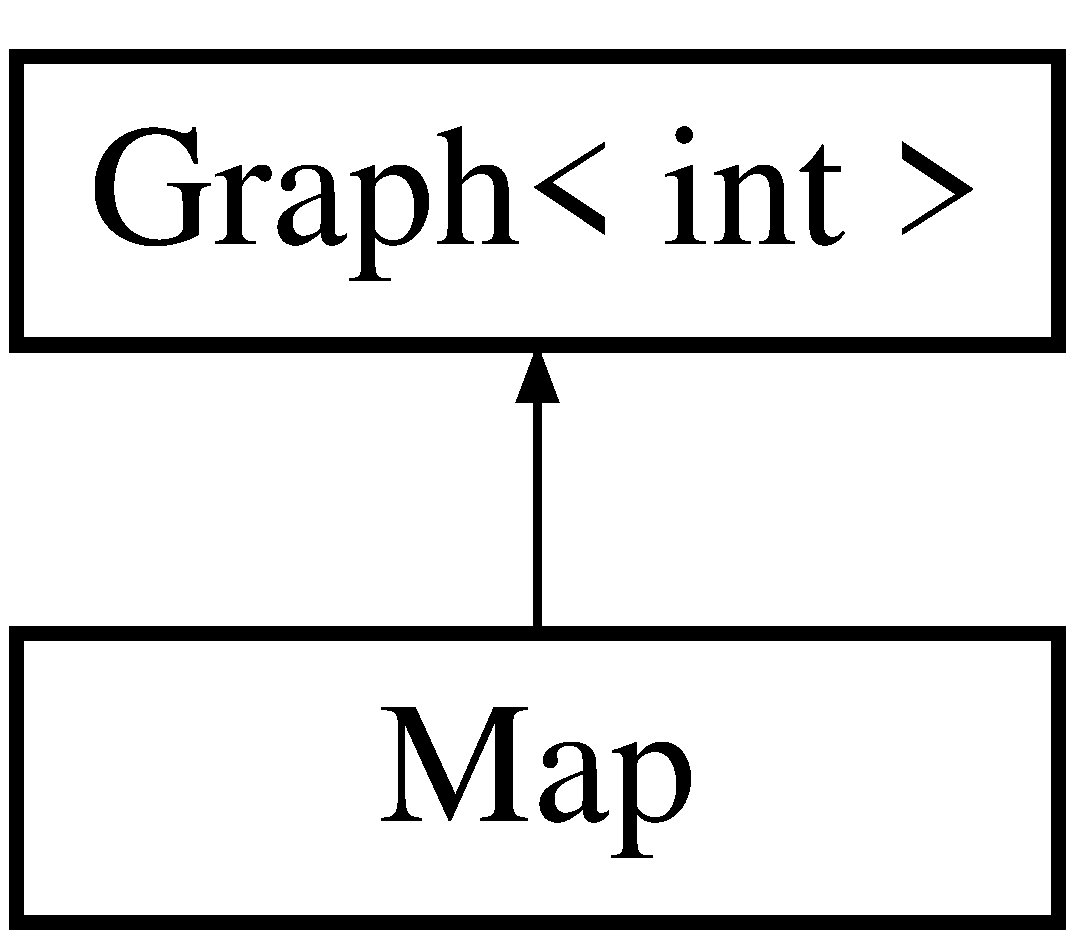
\includegraphics[height=2.000000cm]{classMap}
\end{center}
\end{figure}
\subsection*{Public Member Functions}
\begin{DoxyCompactItemize}
\item 
\hypertarget{classMap_a0f5ad0fd4563497b4214038cbca8b582}{\hyperlink{classMap_a0f5ad0fd4563497b4214038cbca8b582}{Map} ()}\label{classMap_a0f5ad0fd4563497b4214038cbca8b582}

\begin{DoxyCompactList}\small\item\em Empty map constructor. Kind of a placeholder. \end{DoxyCompactList}\item 
bool \hyperlink{classMap_af85ad221d75445dfb341aee1786a3e47}{add\-Vertex} (const int \&in, string name, bool has\-Store)
\begin{DoxyCompactList}\small\item\em Adds a new \hyperlink{classZone}{Zone} to the map. \end{DoxyCompactList}\item 
\hypertarget{classMap_abd12f966840ae67ba28106e13fc92067}{void \hyperlink{classMap_abd12f966840ae67ba28106e13fc92067}{set\-Default} ()}\label{classMap_abd12f966840ae67ba28106e13fc92067}

\begin{DoxyCompactList}\small\item\em Sets the \hyperlink{classMap}{Map} as the default map, adding zones, edges and clients. \end{DoxyCompactList}\item 
int \hyperlink{classMap_a4b728a284793fa3388fd425dcf2d8b09}{choose\-Store} (int d)
\begin{DoxyCompactList}\small\item\em Returns closest store to given zone specified by d. \end{DoxyCompactList}\end{DoxyCompactItemize}
\subsection*{Additional Inherited Members}


\subsection{Detailed Description}
Represents map. Inherits \hyperlink{classGraph}{Graph} class. 

\subsection{Member Function Documentation}
\hypertarget{classMap_af85ad221d75445dfb341aee1786a3e47}{\index{Map@{Map}!add\-Vertex@{add\-Vertex}}
\index{add\-Vertex@{add\-Vertex}!Map@{Map}}
\subsubsection[{add\-Vertex}]{\setlength{\rightskip}{0pt plus 5cm}bool Map\-::add\-Vertex (
\begin{DoxyParamCaption}
\item[{const int \&}]{in, }
\item[{string}]{name, }
\item[{bool}]{has\-Store}
\end{DoxyParamCaption}
)}}\label{classMap_af85ad221d75445dfb341aee1786a3e47}


Adds a new \hyperlink{classZone}{Zone} to the map. 


\begin{DoxyParams}{Parameters}
{\em in} & \hyperlink{classZone}{Zone} I\-D \\
\hline
{\em name} & \hyperlink{classZone}{Zone} name \\
\hline
{\em has\-Store} & Indicates if the \hyperlink{classZone}{Zone} has a store \\
\hline
\end{DoxyParams}
\begin{DoxyReturn}{Returns}
True if insertion successful. False if not successful. 
\end{DoxyReturn}
\hypertarget{classMap_a4b728a284793fa3388fd425dcf2d8b09}{\index{Map@{Map}!choose\-Store@{choose\-Store}}
\index{choose\-Store@{choose\-Store}!Map@{Map}}
\subsubsection[{choose\-Store}]{\setlength{\rightskip}{0pt plus 5cm}int Map\-::choose\-Store (
\begin{DoxyParamCaption}
\item[{int}]{d}
\end{DoxyParamCaption}
)}}\label{classMap_a4b728a284793fa3388fd425dcf2d8b09}


Returns closest store to given zone specified by d. 


\begin{DoxyParams}{Parameters}
{\em d} & Given zone \\
\hline
\end{DoxyParams}
\begin{DoxyReturn}{Returns}
Closest zone I\-D 
\end{DoxyReturn}


The documentation for this class was generated from the following files\-:\begin{DoxyCompactItemize}
\item 
Map.\-h\item 
Map.\-cpp\end{DoxyCompactItemize}

\hypertarget{classVertex}{\section{Vertex$<$ T $>$ Class Template Reference}
\label{classVertex}\index{Vertex$<$ T $>$@{Vertex$<$ T $>$}}
}
\subsection*{Public Member Functions}
\begin{DoxyCompactItemize}
\item 
\hypertarget{classVertex_afcbdd4d4198b672356559cb8fa088408}{{\bfseries Vertex} (T in)}\label{classVertex_afcbdd4d4198b672356559cb8fa088408}

\item 
\hypertarget{classVertex_aeb024eced2da142912f189af6a454db3}{void {\bfseries add\-Edge} (\hyperlink{classVertex}{Vertex}$<$ T $>$ $\ast$dest, double w)}\label{classVertex_aeb024eced2da142912f189af6a454db3}

\item 
\hypertarget{classVertex_a4cab9e6138665f498b1688359e50c241}{void {\bfseries add\-Edge} (\hyperlink{classVertex}{Vertex}$<$ T $>$ $\ast$dest, double w, double f)}\label{classVertex_a4cab9e6138665f498b1688359e50c241}

\item 
\hypertarget{classVertex_ab2b5b43fb1709a901b78718436763a84}{bool {\bfseries remove\-Edge\-To} (\hyperlink{classVertex}{Vertex}$<$ T $>$ $\ast$d)}\label{classVertex_ab2b5b43fb1709a901b78718436763a84}

\item 
\hypertarget{classVertex_a5880b4b252ae6818819c2f9645784b59}{T {\bfseries get\-Info} () const }\label{classVertex_a5880b4b252ae6818819c2f9645784b59}

\item 
\hypertarget{classVertex_a31cd60c26640f8072a928ba70eb2f95e}{void {\bfseries set\-Info} (T info)}\label{classVertex_a31cd60c26640f8072a928ba70eb2f95e}

\item 
\hypertarget{classVertex_a3379c6cbcf1eaacc098381e3557a0b52}{int {\bfseries get\-Dist} () const }\label{classVertex_a3379c6cbcf1eaacc098381e3557a0b52}

\item 
\hypertarget{classVertex_a305ef01582f945f22134abb9294fe1f3}{int {\bfseries get\-Indegree} () const }\label{classVertex_a305ef01582f945f22134abb9294fe1f3}

\item 
\hypertarget{classVertex_a4d8021f4861cc4195af3ecf042a015cc}{vector$<$ \hyperlink{classEdge}{Edge}$<$ T $>$ $>$ {\bfseries get\-Adj} () const }\label{classVertex_a4d8021f4861cc4195af3ecf042a015cc}

\item 
\hypertarget{classVertex_ae0b57c953450db1679e5f5994e1ba738}{\hyperlink{classVertex}{Vertex}$<$ T $>$ $\ast$ {\bfseries get\-Path} () const }\label{classVertex_ae0b57c953450db1679e5f5994e1ba738}

\item 
\hypertarget{classVertex_a7091b26f281a5041b1775a3d3f9cb7a6}{bool {\bfseries operator$<$} (const \hyperlink{classVertex}{Vertex}$<$ T $>$ vertex)}\label{classVertex_a7091b26f281a5041b1775a3d3f9cb7a6}

\item 
\hypertarget{classVertex_abc0db834c5ea38fa4ceb20f231040e7b}{void {\bfseries update\-Edge\-Flow} (unsigned int index, float f)}\label{classVertex_abc0db834c5ea38fa4ceb20f231040e7b}

\end{DoxyCompactItemize}
\subsection*{Public Attributes}
\begin{DoxyCompactItemize}
\item 
\hypertarget{classVertex_a415d7811eef6cdd992f0dca1f35a49cd}{T {\bfseries info}}\label{classVertex_a415d7811eef6cdd992f0dca1f35a49cd}

\item 
\hypertarget{classVertex_a5d9dfdd2caee11e300ff5142799345a1}{vector$<$ \hyperlink{classEdge}{Edge}$<$ T $>$ $>$ {\bfseries adj}}\label{classVertex_a5d9dfdd2caee11e300ff5142799345a1}

\item 
\hypertarget{classVertex_ae575d4b9a6b1ada3f9626c458c060f54}{bool {\bfseries processing}}\label{classVertex_ae575d4b9a6b1ada3f9626c458c060f54}

\item 
\hypertarget{classVertex_a08a2b813e77f97aa8b6c1d252e5417f7}{double {\bfseries dist}}\label{classVertex_a08a2b813e77f97aa8b6c1d252e5417f7}

\item 
\hypertarget{classVertex_abd40febd917aa25add6bd42237c8463a}{\hyperlink{classVertex}{Vertex} $\ast$ {\bfseries path}}\label{classVertex_abd40febd917aa25add6bd42237c8463a}

\end{DoxyCompactItemize}
\subsection*{Friends}
\begin{DoxyCompactItemize}
\item 
\hypertarget{classVertex_aefa9b76cd57411c5354e5620dc2d84dd}{class {\bfseries Graph$<$ T $>$}}\label{classVertex_aefa9b76cd57411c5354e5620dc2d84dd}

\end{DoxyCompactItemize}


The documentation for this class was generated from the following file\-:\begin{DoxyCompactItemize}
\item 
Graph.\-h\end{DoxyCompactItemize}

\hypertarget{structvertex__greater__than}{\section{vertex\-\_\-greater\-\_\-than$<$ T $>$ Struct Template Reference}
\label{structvertex__greater__than}\index{vertex\-\_\-greater\-\_\-than$<$ T $>$@{vertex\-\_\-greater\-\_\-than$<$ T $>$}}
}
\subsection*{Public Member Functions}
\begin{DoxyCompactItemize}
\item 
\hypertarget{structvertex__greater__than_af58940d572829488c2915ca53663631e}{bool {\bfseries operator()} (\hyperlink{classVertex}{Vertex}$<$ T $>$ $\ast$a, \hyperlink{classVertex}{Vertex}$<$ T $>$ $\ast$b) const }\label{structvertex__greater__than_af58940d572829488c2915ca53663631e}

\end{DoxyCompactItemize}


The documentation for this struct was generated from the following file\-:\begin{DoxyCompactItemize}
\item 
Graph.\-h\end{DoxyCompactItemize}

\hypertarget{classZone}{\section{Zone Class Reference}
\label{classZone}\index{Zone@{Zone}}
}


Represents a \hyperlink{classZone}{Zone} in which there may or may not be a store.  




{\ttfamily \#include $<$Zone.\-h$>$}

Inheritance diagram for Zone\-:\begin{figure}[H]
\begin{center}
\leavevmode
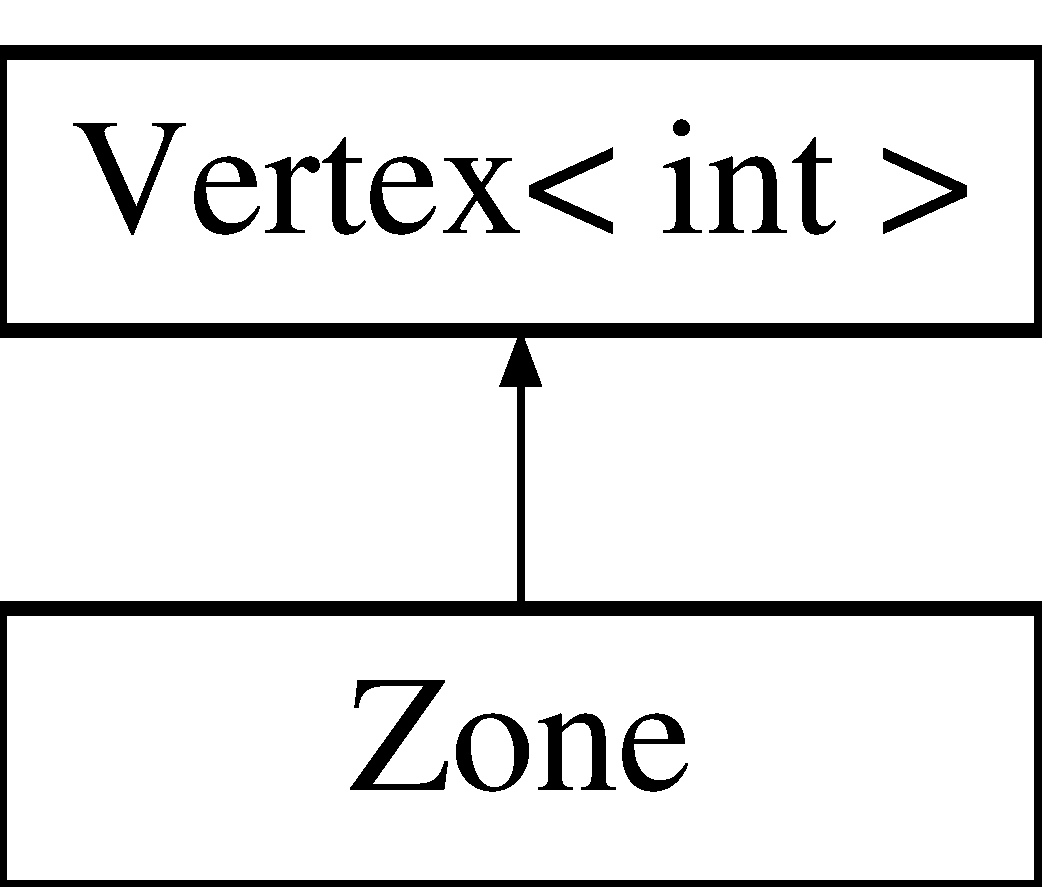
\includegraphics[height=2.000000cm]{classZone}
\end{center}
\end{figure}
\subsection*{Public Member Functions}
\begin{DoxyCompactItemize}
\item 
\hyperlink{classZone_a240ae395a9b19a9822667772f7fa3b28}{Zone} (const int \&in, string name, bool has\-Store)
\begin{DoxyCompactList}\small\item\em \hyperlink{classZone}{Zone} constructor. \end{DoxyCompactList}\item 
void \hyperlink{classZone_a2a3407fdaaaa3926be04cdf7294750ac}{add\-Client} (\hyperlink{classClient}{Client} c)
\begin{DoxyCompactList}\small\item\em Adds a client to the \hyperlink{classZone}{Zone} client vector. \end{DoxyCompactList}\item 
\hypertarget{classZone_a4af37f9d0b95ac5efd5930c5d3a237bf}{void {\bfseries remove\-Client} (unsigned long N\-I\-F)}\label{classZone_a4af37f9d0b95ac5efd5930c5d3a237bf}

\item 
bool \hyperlink{classZone_ac96cd131db38f2e28da929a7f7b0db00}{check\-Store} ()
\begin{DoxyCompactList}\small\item\em Checks if the \hyperlink{classZone}{Zone} has a store. \end{DoxyCompactList}\item 
string \hyperlink{classZone_a94bcfd6622d27041130bb1d56021e557}{get\-Name} ()
\begin{DoxyCompactList}\small\item\em Checks if the \hyperlink{classZone}{Zone} has a store. \end{DoxyCompactList}\item 
void \hyperlink{classZone_afffd33b4006d092866f9cd99d67070c4}{set\-Store} (bool has\-Store)
\begin{DoxyCompactList}\small\item\em Sets the store status in a \hyperlink{classZone}{Zone}. \end{DoxyCompactList}\item 
int \hyperlink{classZone_a40d5df046e49023ac0f9376c645573b2}{get\-I\-D} ()
\begin{DoxyCompactList}\small\item\em Checks if the \hyperlink{classZone}{Zone} has a store. \end{DoxyCompactList}\end{DoxyCompactItemize}
\subsection*{Static Public Member Functions}
\begin{DoxyCompactItemize}
\item 
\hypertarget{classZone_a334033d0188c5ad5d79e1940e468a667}{static void \hyperlink{classZone_a334033d0188c5ad5d79e1940e468a667}{reset\-I\-D} ()}\label{classZone_a334033d0188c5ad5d79e1940e468a667}

\begin{DoxyCompactList}\small\item\em Resets I\-D counter. Used when graph is loaded. \end{DoxyCompactList}\end{DoxyCompactItemize}
\subsection*{Public Attributes}
\begin{DoxyCompactItemize}
\item 
\hypertarget{classZone_a6a9280bd93f5f5edd83c57cec77fdcd6}{vector$<$ \hyperlink{classClient}{Client} $>$ {\bfseries clients}}\label{classZone_a6a9280bd93f5f5edd83c57cec77fdcd6}

\item 
\hypertarget{classZone_a2a23da1e70eea3831a0fa1901e47e342}{bool {\bfseries has\-Store}}\label{classZone_a2a23da1e70eea3831a0fa1901e47e342}

\end{DoxyCompactItemize}
\subsection*{Friends}
\begin{DoxyCompactItemize}
\item 
\hypertarget{classZone_ad2f32e921244459f7cc6d50355429cc6}{class {\bfseries Map}}\label{classZone_ad2f32e921244459f7cc6d50355429cc6}

\end{DoxyCompactItemize}


\subsection{Detailed Description}
Represents a \hyperlink{classZone}{Zone} in which there may or may not be a store. 

\subsection{Constructor \& Destructor Documentation}
\hypertarget{classZone_a240ae395a9b19a9822667772f7fa3b28}{\index{Zone@{Zone}!Zone@{Zone}}
\index{Zone@{Zone}!Zone@{Zone}}
\subsubsection[{Zone}]{\setlength{\rightskip}{0pt plus 5cm}Zone\-::\-Zone (
\begin{DoxyParamCaption}
\item[{const int \&}]{in, }
\item[{string}]{name, }
\item[{bool}]{has\-Store}
\end{DoxyParamCaption}
)}}\label{classZone_a240ae395a9b19a9822667772f7fa3b28}


\hyperlink{classZone}{Zone} constructor. 


\begin{DoxyParams}{Parameters}
{\em in} & \hyperlink{classVertex}{Vertex} I\-D \\
\hline
{\em name} & \hyperlink{classZone}{Zone} name \\
\hline
{\em has\-Store} & Indicates if the \hyperlink{classZone}{Zone} has a store \\
\hline
\end{DoxyParams}


\subsection{Member Function Documentation}
\hypertarget{classZone_a2a3407fdaaaa3926be04cdf7294750ac}{\index{Zone@{Zone}!add\-Client@{add\-Client}}
\index{add\-Client@{add\-Client}!Zone@{Zone}}
\subsubsection[{add\-Client}]{\setlength{\rightskip}{0pt plus 5cm}void Zone\-::add\-Client (
\begin{DoxyParamCaption}
\item[{{\bf Client}}]{c}
\end{DoxyParamCaption}
)}}\label{classZone_a2a3407fdaaaa3926be04cdf7294750ac}


Adds a client to the \hyperlink{classZone}{Zone} client vector. 


\begin{DoxyParams}{Parameters}
{\em c} & The client \\
\hline
\end{DoxyParams}
\hypertarget{classZone_ac96cd131db38f2e28da929a7f7b0db00}{\index{Zone@{Zone}!check\-Store@{check\-Store}}
\index{check\-Store@{check\-Store}!Zone@{Zone}}
\subsubsection[{check\-Store}]{\setlength{\rightskip}{0pt plus 5cm}bool Zone\-::check\-Store (
\begin{DoxyParamCaption}
{}
\end{DoxyParamCaption}
)}}\label{classZone_ac96cd131db38f2e28da929a7f7b0db00}


Checks if the \hyperlink{classZone}{Zone} has a store. 

\begin{DoxyReturn}{Returns}
True if the \hyperlink{classZone}{Zone} has a store. False if the zone has no store. 
\end{DoxyReturn}
\hypertarget{classZone_a40d5df046e49023ac0f9376c645573b2}{\index{Zone@{Zone}!get\-I\-D@{get\-I\-D}}
\index{get\-I\-D@{get\-I\-D}!Zone@{Zone}}
\subsubsection[{get\-I\-D}]{\setlength{\rightskip}{0pt plus 5cm}int Zone\-::get\-I\-D (
\begin{DoxyParamCaption}
{}
\end{DoxyParamCaption}
)}}\label{classZone_a40d5df046e49023ac0f9376c645573b2}


Checks if the \hyperlink{classZone}{Zone} has a store. 

\begin{DoxyReturn}{Returns}
True if the \hyperlink{classZone}{Zone} has a store. False if the zone has no store. 
\end{DoxyReturn}
\hypertarget{classZone_a94bcfd6622d27041130bb1d56021e557}{\index{Zone@{Zone}!get\-Name@{get\-Name}}
\index{get\-Name@{get\-Name}!Zone@{Zone}}
\subsubsection[{get\-Name}]{\setlength{\rightskip}{0pt plus 5cm}string Zone\-::get\-Name (
\begin{DoxyParamCaption}
{}
\end{DoxyParamCaption}
)}}\label{classZone_a94bcfd6622d27041130bb1d56021e557}


Checks if the \hyperlink{classZone}{Zone} has a store. 

\begin{DoxyReturn}{Returns}
True if the \hyperlink{classZone}{Zone} has a store. False if the zone has no store. 
\end{DoxyReturn}
\hypertarget{classZone_afffd33b4006d092866f9cd99d67070c4}{\index{Zone@{Zone}!set\-Store@{set\-Store}}
\index{set\-Store@{set\-Store}!Zone@{Zone}}
\subsubsection[{set\-Store}]{\setlength{\rightskip}{0pt plus 5cm}void Zone\-::set\-Store (
\begin{DoxyParamCaption}
\item[{bool}]{has\-Store}
\end{DoxyParamCaption}
)}}\label{classZone_afffd33b4006d092866f9cd99d67070c4}


Sets the store status in a \hyperlink{classZone}{Zone}. 


\begin{DoxyParams}{Parameters}
{\em has\-Store} & Store status. \\
\hline
\end{DoxyParams}


The documentation for this class was generated from the following files\-:\begin{DoxyCompactItemize}
\item 
Zone.\-h\item 
Zone.\-cpp\end{DoxyCompactItemize}

\addcontentsline{toc}{part}{Index}
\printindex
\end{document}
